\documentclass{article}%
\usepackage[T1]{fontenc}%
\usepackage[utf8]{inputenc}%
\usepackage{lmodern}%
\usepackage{textcomp}%
\usepackage{lastpage}%
\usepackage{authblk}%
\usepackage{graphicx}%
%
\title{Pathological Impact of Hepatitis B Virus Surface Proteins on the Liver Is Associated with the Host Genetic Background}%
\author{Debra Kennedy}%
\affil{Department of Oral Biology and Pathology, School of Dental Medicine, Stony Brook University, Stony Brook, New York, United States of America}%
\date{01{-}01{-}2012}%
%
\begin{document}%
\normalsize%
\maketitle%
\section{Abstract}%
\label{sec:Abstract}%
Caffeic acid can boost the production of a key signaling molecule in cancer cells, according to new research published online in the journal Cell Metabolism.\newline%
In a heart{-}shaped tube created by a patient's own cells, the researchers removed the tumor tissue and exposed the cells to powerful antibiotics. When they removed cancerous cells, they saw that the cancer cells didn't respond well to the antibiotics. But when exposed to the analgesic compound erazine, however, the cell survived.\newline%
The researchers found the cancer cells took up the erazine and released it. The cancer cells left the cancer cells with the erazine. Erazine caused the cancer cells to become slower to attack, resulting in the death of many cancer cells, and a "normal" life for the cancer cells.\newline%
"Caffeic acid is the most commonly used cancer suppressor drug in the marketplace," said Pramod Rao, M.D., an American College of Clinical Oncology Fellow in the Department of hematology/oncology, University of Texas Medical Branch at Galveston and senior author of the study. "It is the principal inhibitor of angiogenesis and just as important for the cell's survival."\newline%
If more research is completed, the researchers hope that a drug called erazine may be effective against patients with myelofibrosis, a disease in which bones develop disfiguring fractures.

%
\subsection{Image Analysis}%
\label{subsec:ImageAnalysis}%


\begin{figure}[h!]%
\centering%
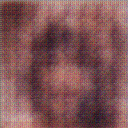
\includegraphics[width=150px]{500_fake_images/samples_5_190.png}%
\caption{A Close Up Of A Small Bird In A Field}%
\end{figure}

%
\end{document}